\chapter{Description of the measurement procedures}
\label{sec:measurement}
The simplified schematic of a Input/Output-Port pin of the ATmega is shown in figure~\ref{fig:port}.
The PUD switch isolates all ``pull up'' resistors of the ATmega. The output of a pin can be switched off
with the DD switch. The Input can operate regardless to the state of the switch DD.
The PORT switch usually defined the output level, but also switches the pull up resistor.
Because the Switches PORT and DD can not be changed at the same time but only one after another, the
pull up resistors can disturb the measurement. Therefore I prefere to disable the pull up resistors with the
PUD switch.
Of course all the switches are electronic type and the resistors \(19\Omega\) and \(22\Omega\) are approximated values.

\begin{figure}[H]
\centering
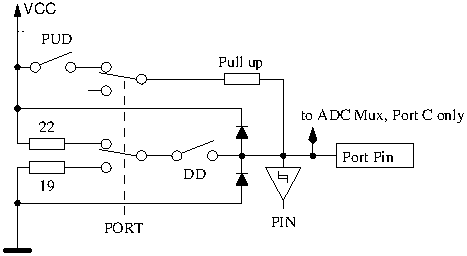
\includegraphics[]{../FIG/port.pdf}
\caption{simplified diagram of each ATmega port pin}
\label{fig:port}
\end{figure}

Every of the three terminal probes of your Transistor Tester is build with three ATmega port pins,
which is shown as simplified diagram for the terminal probe TP2 (middle of three pins) in figure~\ref{fig:terminal}.

\begin{figure}[H]
\centering
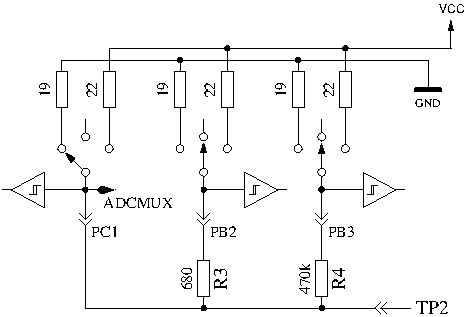
\includegraphics[]{../FIG/terminal.pdf}
\caption{simplified circuit of each measurement terminal probe TP}
\label{fig:terminal}
\end{figure}

Every test pin (measurement port) can be used as digital or analog input. This measurement capability is
independent of using the port as output.
Every test pin can be switched to output and in this mode it can be directly connected to GND (\(0V\)) or VCC (\(5V\)), 
or it can be connected via a \(680\Omega\) resistor or a \(470k\Omega\) resistor to either GND or VCC.
Table \ref{tab:case} shows all possible combination of measurements.
Notice, that the positive state can be switched directly to VCC (Port C) or it can be connected with the 
\(680\Omega\) resistor to VCC (Port B). The same possibility has the negative state of terminal probe to the GND side.
The test state means, that probe can be open (Input), connected with the \(470k\Omega\) resistor to VCC or GND,
or that the probe can be connected with the \(680\Omega\) resistor to VCC or GND.

\begin{table}[H]
  \begin{center}
    \begin{tabular}{| l | c | c | c |}
    \hline
      & state pin 1 & state pin 2 & state pin 3 \\
    \hline
   1. & positive    &  negative    &  test \\
   2. & positive    &  test       & negative \\
   3. & test        &  negative    & positive \\
   4. & test        &  positive    & negative \\
   5. & negative     &  test       & positive \\
   6. & negative     &  positive    &  test  \\
    \hline
    \end{tabular}
  \end{center}
  \caption{all combinations of measurement}
  \label{tab:case} 
\end{table}

If the capacitor measuring is configured for the tester, the tester will try to discharge the capacitors connected at all
test pins.
If discharge will fail, that means the remaining voltage is to high, the discharging will be aborted after about 12 seconds
with the meassage ''Cell!''. This can also be happen, if no capacitor is connected to any test pin.
The cause for this can be, that the cut-off voltage is choosed to low for this ATmega.
You can choose a higher voltage with the Makefile option CAP\_EMPTY\_LEVEL.
